\documentclass{beamer}
\usepackage{listings}
\lstset{
%language=C,
frame=single, 
breaklines=true,
columns=fullflexible
}
\usepackage{gensymb}
\usepackage{subcaption}
\usepackage{url}
\usepackage{tikz}
\usepackage{tkz-euclide} % loads  TikZ and tkz-base
%\usetkzobj{all}
\usetikzlibrary{calc,math}
\usepackage{float}
\newcommand{\myvec}[1]{\ensuremath{\begin{pmatrix}#1\end{pmatrix}}}
\providecommand{\brak}[1]{\ensuremath{\left(#1\right)}}
\newcommand\norm[1]{\left\lVert#1\right\rVert}
\renewcommand{\vec}[1]{\mathbf{#1}}
\providecommand{\abs}[1]{\vert#1\vert}
\usepackage[export]{adjustbox}
\usepackage[utf8]{inputenc}
\usepackage{amsmath}
\usepackage{amssymb}
\usepackage{mathtools}
\usetheme{Boadilla}
\providecommand{\pr}[1]{\ensuremath{\Pr\left(#1\right)}}
\newcommand{\mydet}[1]{\ensuremath{\begin{vmatrix}#1\end{vmatrix}}}

\title{Assignment 4 Presentation}
\author{Yashas Tadikamalla}
\date{AI20BTECH11027}
\begin{document}

\begin{frame}
\titlepage
\end{frame}

\begin{frame}
\frametitle{Question}
\begin{block}{Problem (Linear Forms Q2.33)}
If the lines
$$\dfrac{x-1}{-3}=\dfrac{y-2}{2k}=\dfrac{z-3}{2}$$
$$\dfrac{x-3}{3k}=\dfrac{y-1}{1}=\dfrac{z-6}{-5}$$
are coplanar, find the value of $k$.
\end{block}
\end{frame}



\begin{frame}
\frametitle{Solution}
Given, two coplanar lines,
\begin{align}
\dfrac{x-1}{-3}=\dfrac{y-2}{2k}=\dfrac{z-3}{2}\\
\dfrac{x-3}{3k}=\dfrac{y-1}{1}=\dfrac{z-6}{-5}
\end{align}
For them,
\begin{align}
    \vec{m_{1}}&=\myvec{-3\\
    2k\\
    2}, \vec{m_{2}}=\myvec{3k\\
    1\\
    -5}\\
    \vec{A_{1}}&=\myvec{1\\
    2\\
    3}, \vec{A_{2}}=\myvec{3\\
    1\\
    6}
\end{align}
where $\vec{m_{1}},\vec{m_{2}}$ are the respective direction vectors and $\vec{A_{1}},\vec{A_{2}}$ are the respective points through which the lines pass.
\end{frame}

\begin{frame}
\frametitle{Solution Contd.}
As the lines are given to be coplanar, they are either parallel or intersecting.
Let's check if our lines are parallel. Consider the matrix
\begin{align}
    \myvec{-3 & 2k & 2 \\
    3k & 1 & -5}
\end{align}
If the lines are parallel, the $rank$ of the above matrix will be 1.
\begin{align}
    \Rightarrow \mydet{-3 & 2k \\
    3k & 1} &=0\\
    \Rightarrow 6k^{2}+3&=0
\end{align}
This is not possible. Hence, the lines must cannot be parallel. That means the lines must be intersecting.
\end{frame}

\begin{frame}
\frametitle{Solution Contd.}
That means the lines must be intersecting. In that case,
\begin{align}
    \brak{\vec{A_{1}}-\vec{A_{2}}}^{T}\brak{\vec{m_{1}}\times\vec{m_{2}}}=0\label{eq:a}
\end{align}
$\vec{m_{1}}\times\vec{m_{2}}$ is obtained by row reducing the matrix,
\begin{align}
    &\myvec{-3 & 2k & 2 \\
    3k & 1 & -5}\xleftrightarrow {R_2\leftarrow\frac{R_2+kR_1}{1+2k^2}}\myvec{-3 & 2k & 2 \\
    0 & 1 & \frac{2k-5}{1+2k^{2}}}\\
    &\xleftrightarrow {R_1\leftarrow \frac{R_1-2kR_2}{-3}}\myvec{1 & 0 & \frac{10k+2}{-3(1+2k^{2})} \\
    0 & 1 & \frac{2k-5}{1+2k^{2}}}
\end{align}
\end{frame}

\begin{frame}
\frametitle{Solution Contd.}
Substituting in \eqref{eq:a},
\begin{align}
    \myvec{-2\\1\\-3}^{T}\myvec{\frac{10k+2}{3(1+2k^{2})}\\\frac{5-2k}{1+2k^{2}}\\1}&=0\\
    \Rightarrow -\frac{20k+4}{3+6k^{2}}+\frac{5-2k}{1+2k^{2}}&=3\\
    \Rightarrow \frac{11-26k}{3+6k^{2}}&=3\\
    \Rightarrow 9k^2+13k-1&=0\label{eq:quad}
\end{align}
Solving this, we get
\begin{align}
    k&=\dfrac{-13\pm \sqrt{205}}{18}
\end{align}
For the above values of $k$, the lines are intersecting, and hence, coplanar.
\end{frame}

\begin{frame}
\frametitle{Solution Contd.}
The lines can be rewritten as
\begin{align}
    \vec{x}=\vec{A_{1}}+\lambda_{1}\vec{m_{1}}\label{eq:form}\\
    \vec{x}=\vec{A_{2}}+\lambda_{2}\vec{m_{1}}
\end{align}
The point of intersection can be found by equating them
\begin{align}
    \vec{A_{1}}+\lambda_{1}\vec{m_{1}}=\vec{A_{2}}+\lambda_{2}\vec{m_{2}}\\
    \vec{A_{1}}-\vec{A_{2}}+\lambda_{1}\vec{m_{1}}-\lambda_{2}\vec{m_{2}}=0\label{eq:2019}
\end{align}
Take $\vec{A}=\vec{A_{1}}-\vec{A_{2}},\vec{\lambda}=\myvec{\lambda_{1}\\\lambda_{2}},\vec{m}=\myvec{\vec{m_{1}} & -\vec{m_{2}}}$. Then, \eqref{eq:2019} can be rewritten as
\begin{align}
    \vec{A}+\vec{m}\vec{\lambda}=0\\
    \Rightarrow\vec{m}\vec{\lambda}=-\vec{A}\label{eq:2020}
\end{align}
\end{frame}

\begin{frame}
\frametitle{Solution Contd.}
Substituting in \eqref{eq:2020}, we get
\begin{align}
    \myvec{-3 & -3k\\
    2k & -1\\
    2 &  5}\myvec{\lambda_{1}\\\lambda_{2}}=\myvec{2\\-1\\3}
\end{align}
The corresponding augmented matrix is 
\begin{align}
    \myvec{-3 & -3k & \vrule & 2\\
    2k & -1 & \vrule & -1\\
    2 &  5 & \vrule & 3}
\end{align}
Row reducing the matrix, we get
\begin{align}
    &\myvec{-3 & -3k & \vrule & 2\\
    2k & -1 & \vrule & -1\\
    2 &  5 & \vrule & 3}\xleftrightarrow{R_1\leftarrow R_{1}+2R_{2}}\myvec{-3+4k & -3k-2 & \vrule & 0\\
    2k & -1 & \vrule & -1\\
    2 &  5 & \vrule & 3}\\
    &\xleftrightarrow{R_3\leftarrow \frac{R_{3}+3R_{2}}{2}}\myvec{-3+4k & -3k-2 & \vrule & 0\\
    2k & -1 & \vrule & -1\\
    1+3k &  1 & \vrule & 0}   
\end{align}
\end{frame}

\begin{frame}
\frametitle{Solution Contd.}
\begin{align}
    \xleftrightarrow{R_1\leftarrow R_1+(3k+2)R_3}\myvec{9k^2+13k-1& 0 & \vrule & 0\\
    2k & -1 & \vrule & -1\\
    1+3k &  1 & \vrule & 0}
\end{align}
Clearly, from \eqref{eq:quad}, it is
\begin{align}
    &\myvec{0 & 0 & \vrule & 0\\
    2k & -1 & \vrule & -1\\
    1+3k &  1 & \vrule & 0}\xleftrightarrow{R_3\leftarrow2R_3}\myvec{0 & 0 & \vrule & 0\\
    2k & -1 & \vrule & -1\\
    2+6k &  2 & \vrule & 0}\\&\xleftrightarrow{R_3\leftarrow R_3-3R_2}\myvec{0 & 0 & \vrule & 0\\
    2k & -1 & \vrule & -1\\
    2 &  5 & \vrule & 3}\xleftrightarrow{R_1\leftarrow R_1+R_3}\myvec{2 & 5 & \vrule & 3\\
    2k & -1 & \vrule & -1\\
    2 &  5 & \vrule & 3}\\&\xleftrightarrow{R_3\leftarrow R_3+R_1}\myvec{2 & 5 & \vrule & 3\\
    2k & -1 & \vrule & -1\\
    0 &  0 & \vrule & 0}
\end{align}
\end{frame}

\begin{frame}
\frametitle{Solution Contd.}
We can observe that, on row reduction, we get a complete row to be $0$. 
\begin{align}
    &\xleftrightarrow{R_1\leftarrow R_{1}+5R_{2}}
	\myvec{2+10k & 0 & \vrule & -2 \\
	2k & -1 & \vrule & -1 \\
	0 & 0 & \vrule & 0}\xleftrightarrow{R_1\leftarrow \frac{R_{1}}{2+10k}}
	\myvec{1 & 0 & \vrule & \frac{-2}{2+10k} \\
	2k & -1 & \vrule & -1 \\
	0 & 0 & \vrule & 0}\\
	&\xleftrightarrow{R_2\leftarrow -R_{2}}
	\myvec{1 & 0 & \vrule & \frac{-2}{2+10k} \\
	-2k & 1 & \vrule & 1 \\
	0 & 0 & \vrule & 0}\xleftrightarrow{R_2\leftarrow R_{2}+2kR_{1}}
	\myvec{1 & 0 & \vrule & \frac{-2}{2+10k} \\
	0 & 1 & \vrule & \frac{6k+2}{2+10k} \\
	0 & 0 & \vrule & 0}\\
	&\therefore \lambda_{1}=\frac{-1}{1+5k},\lambda_{2}=\frac{3k+1}{1+5k}
\end{align}
\end{frame}

\begin{frame}
\frametitle{Solution Contd.}
Substituting $\lambda_{1}$ in \eqref{eq:form} to get the required point of intersection $\vec{P}$,
\begin{align}
    \vec{P}=\myvec{1+\frac{3}{1+5k}\\
    2-\frac{2k}{1+5k}\\
    3-\frac{2}{1+5k}}\Rightarrow \vec{P}=\myvec{\frac{4+5k}{1+5k}\\\\
    \frac{2+8k}{1+5k}\\\\
    \frac{1+15k}{1+5k}}
\end{align}
where $k=\dfrac{-13\pm \sqrt{205}}{18}$.
\end{frame}

\begin{frame}
\frametitle{Solution Contd.}
\begin{figure}[!h]
 \centering
 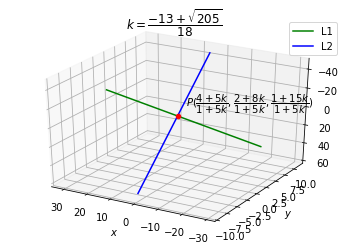
\includegraphics[width=0.75\columnwidth]{Assignment4Presentation(1).png}
 \caption{Intersecting lines - Case1}
 \label{plot}
\end{figure}
\end{frame}

\begin{frame}
\frametitle{Solution Contd.}
\begin{figure}[!h]
 \centering
 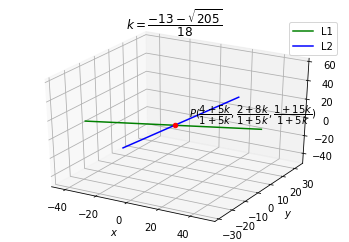
\includegraphics[width=0.75\columnwidth]{Assignment4Presentation(2).png}
 \caption{Intersecting lines - Case2}
 \label{plot}
\end{figure}
\end{frame}
\end{document}